\htwo{Github}\label{sec:github}
\sectionauthor{Johannes Polzer}
\hthree{Allgemein}

Um die aglile Entwickungsmethodig umzusetzten wird Github verwendet. 
Github bietet nicht nur die Möglichkeit den Quellcode mittels Git zu verwalten, sondern auch einzelne Arbeitspakete zu erstellen und diese Meilensteinen und Unterprojekten Zuzuordnen.

Dabei ist es möglich, dass der Status eines einzelnen Arbeitspaketes automatisch bei der Durchführung eines "Pull-Requests in die bei der agilen Entwicklung üblichen Spalten verschoben wird. Diese Spalten sind:

\begin{description}
    \item[To Do] Die Arbeitspakete sind angelegt, werden allerdings noch nicht bearbeitet.
    \item[In Progress] Die Arbeitspakete werden bearbeitet.
    \item[Review in progress] Die Entwicklung an diesem Arbeitspaket ist abgeschlossen, und ein anderer Entwickler muss nach dem vier-Augen-Prinzip den Code überprüfen. 
    \item[Review approved] Der Code wurde überprüft und der Entwickler hat den Code akzeptiert, allerdings ist der Code noch nicht auf den Branch des jeweiligen Sprints geführt worden.
    \item[Done] Der Merge vom Entwicklungsbranch auf den Branch des jeweiligen Sprints wurde durchgeführt.
\end{description}

% TODO: cross ref zu Scrum

\hthree{Erstellen eines Projektes}

Um ein Projekt zu erstellen, muss zunächst ein Projekt im "Projects"-Tab (Abbildung \ref{fig:newProject}) erstellt werden.

\begin{figure}[H]
    \centering
    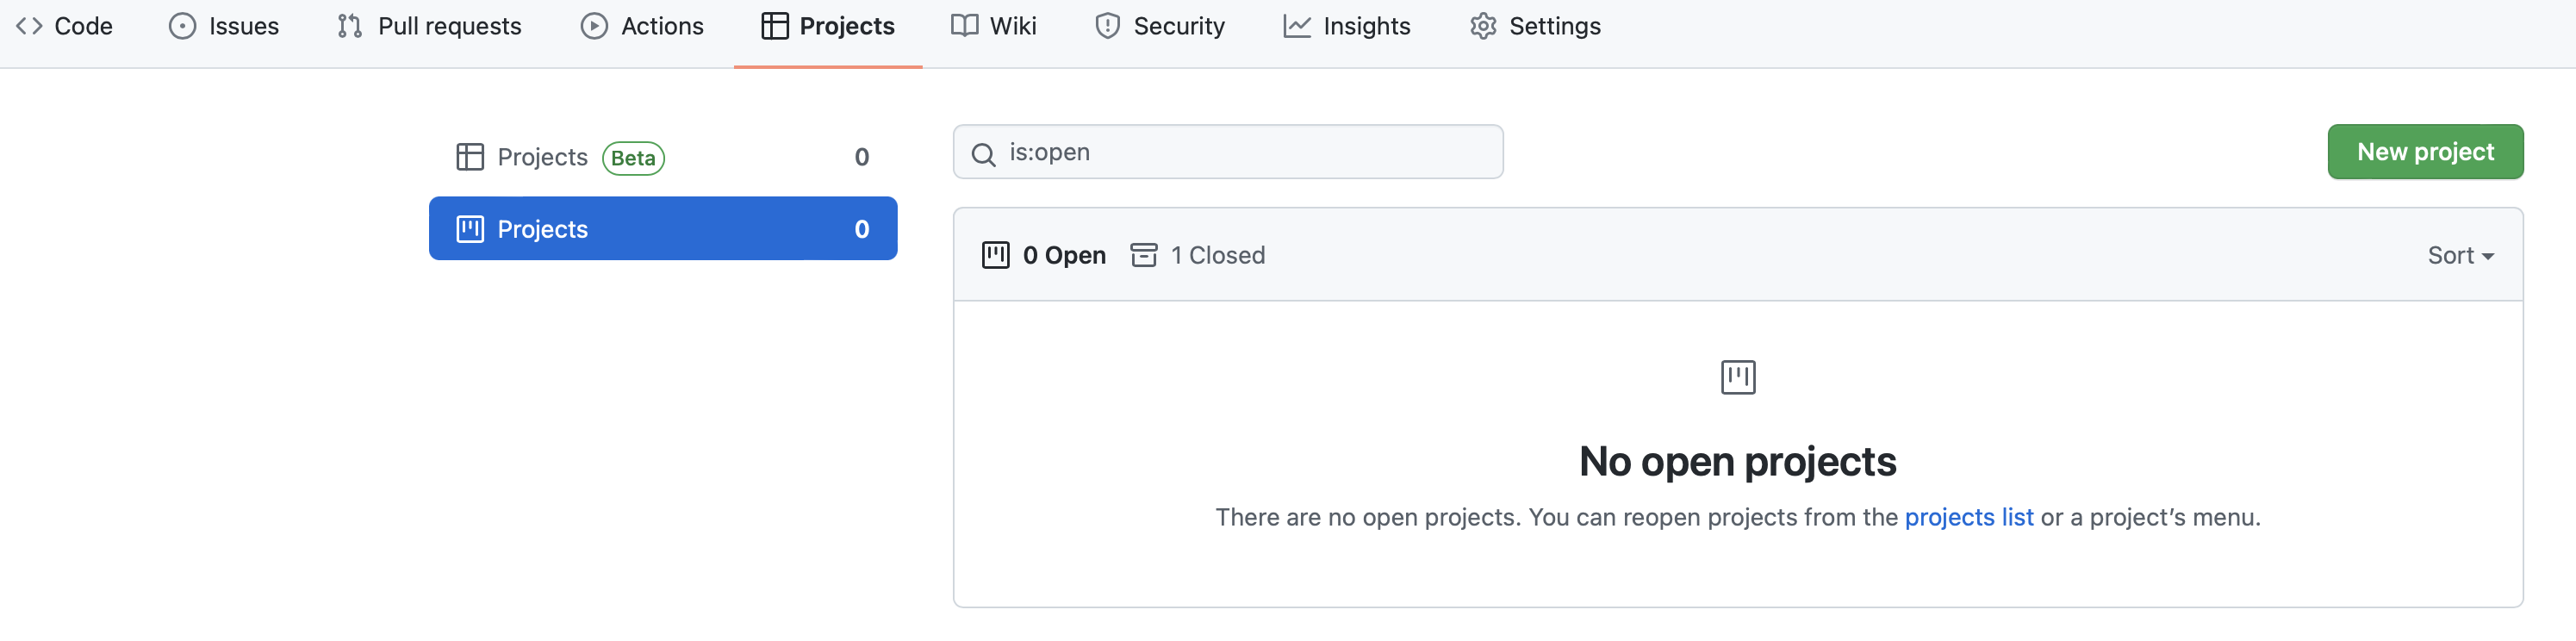
\includegraphics[width=\textwidth]{media/ProjectManagement/CreateProject.png}
    \caption{Github Projektübersicht mit "New Project" Button}
    \label{fig:newProject}
\end{figure}

Einem Projekt wird ein Name und eine Beschreibung zugewiesen. Damit die Spalten für die agile Entwicklung erstellt werden, und die Karten darin automatisch verschoben werden, muss  "Automated kanban with reviews" beim Projekt-"template" ausgewählt werden (siehe Abbildung \ref{fig:enterProjectInfo}).

\begin{figure}[H]
    \centering
    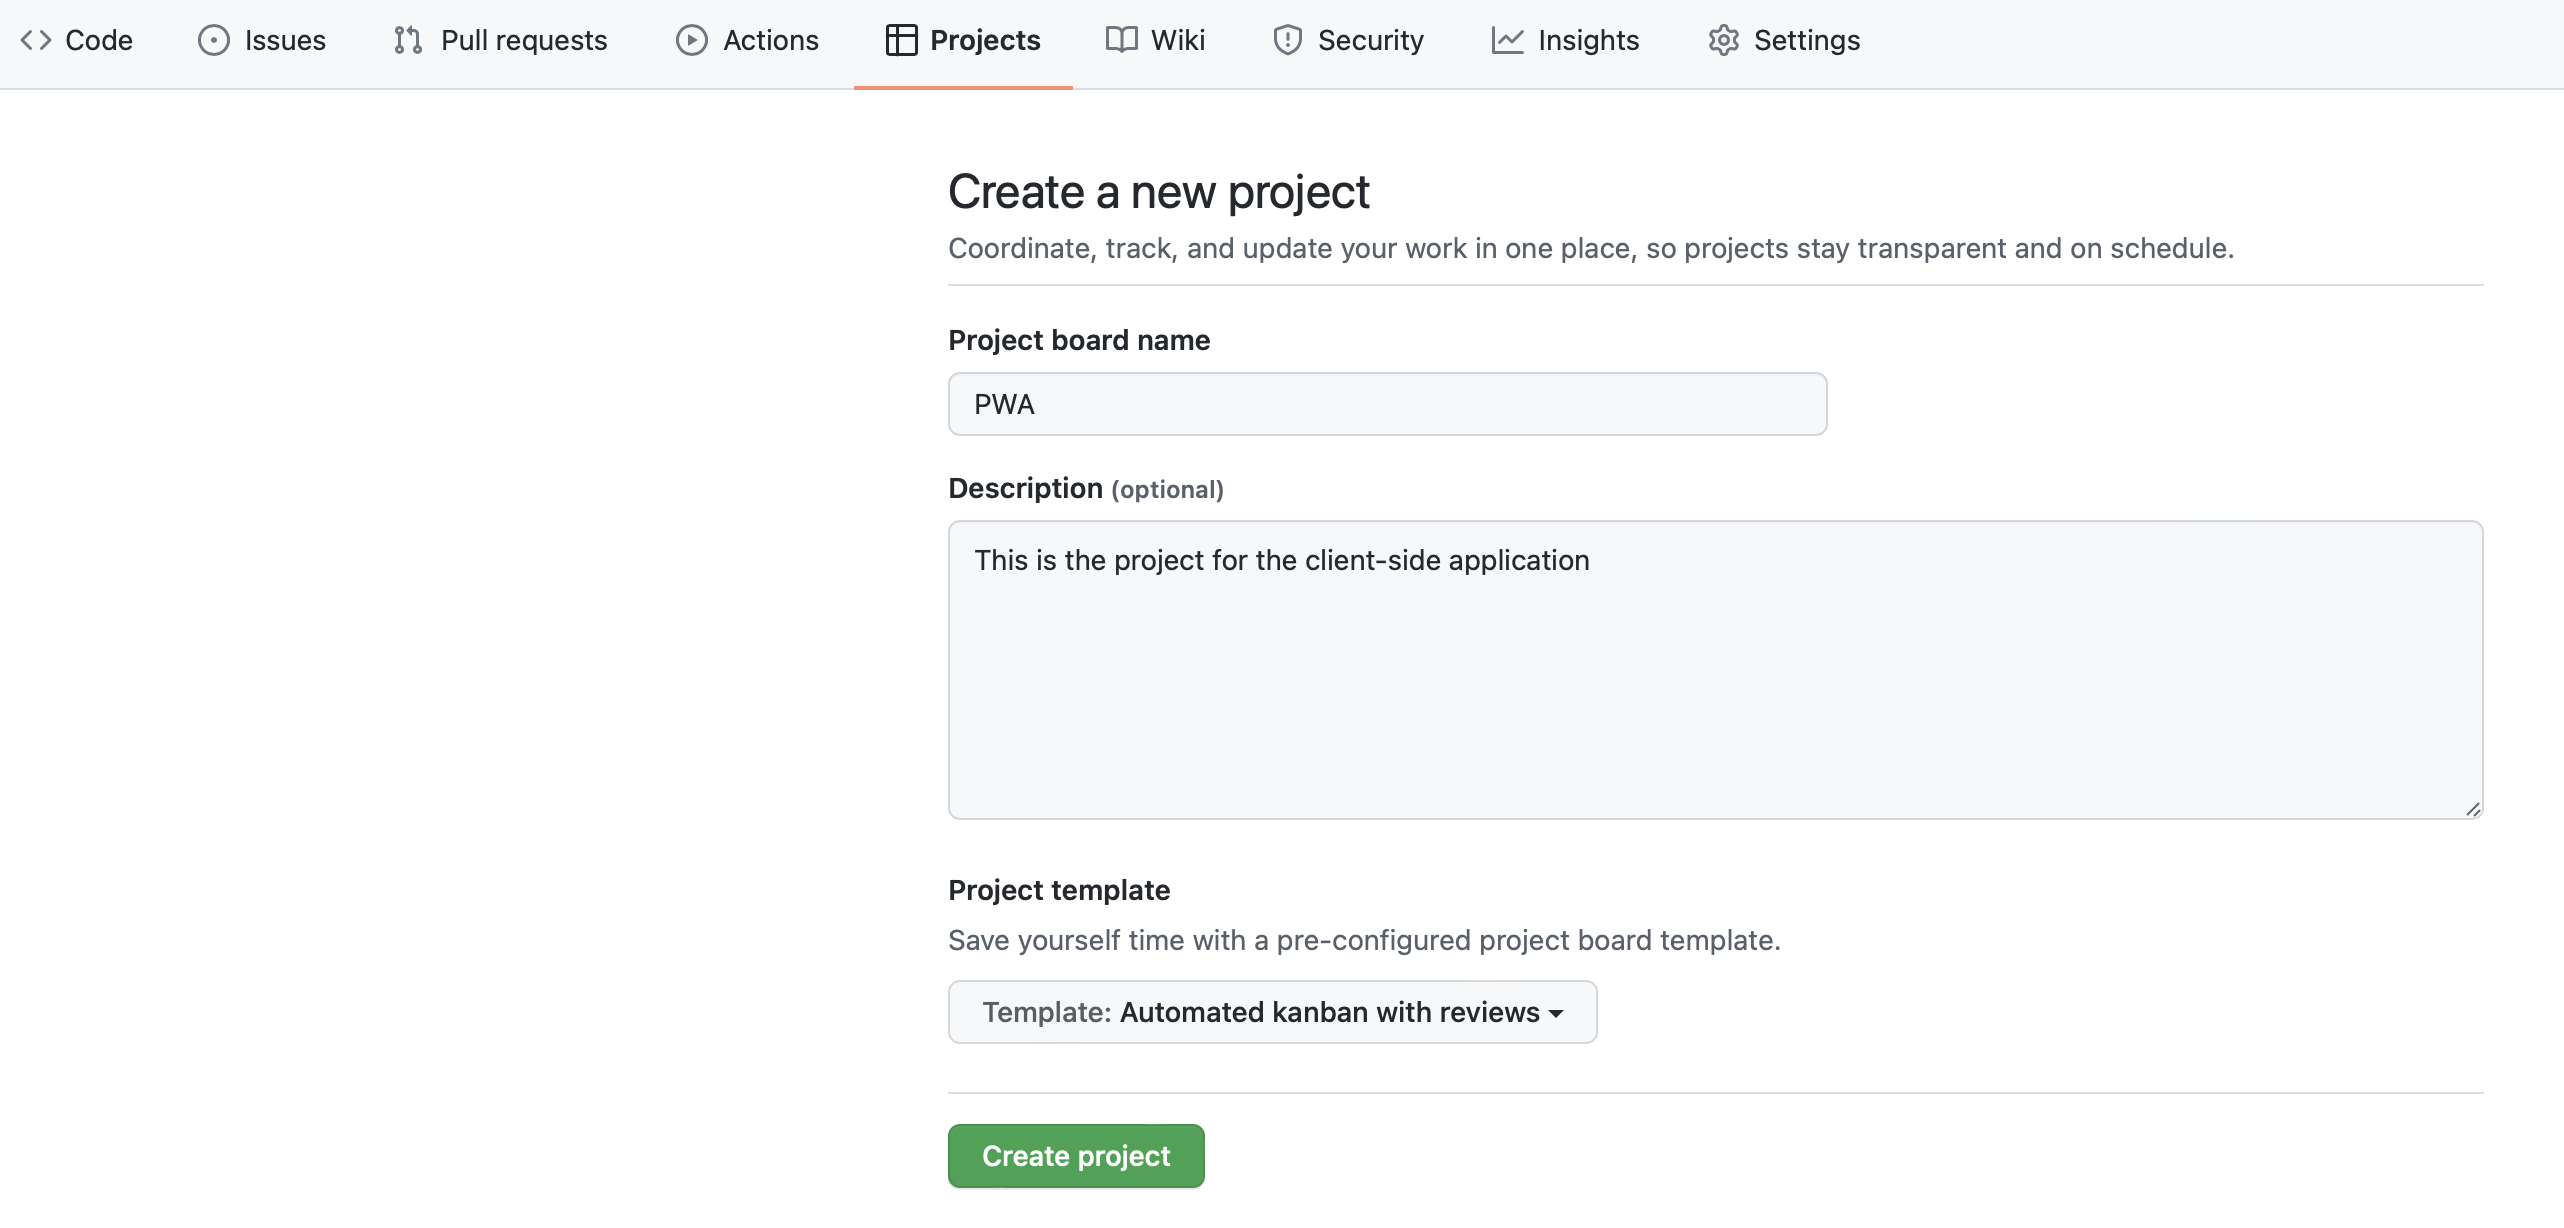
\includegraphics[width=\textwidth]{media/ProjectManagement/EnterProjectInfo.png}
    \caption{Eingabe der Projektinformationen (Demo-Bild)}
    \label{fig:enterProjectInfo}
\end{figure}

\hthree{Erstellen eines Arbeitspaketes}

Arbeitspaket werden im "Issues"-Tab erstellt. In jedem "Issue" wird ein Titel und eine Beschreibung eingetragen. Außerdem können Label, Meilensteine und verantwortliche Entwickler zugewiesen werden (siehe Abbildung \ref{fig:createIssue}). 

Meilensteine sind zeitliche Ziele, und können somit als das Ziel eines "Sprints" bezeichnet werden. Diese können ebenfalls im "Issues"-Tab erstellt werden.

Durch "Label" wird die Art des Arbeitspaketes definiert. Bei Github gibt es vorgefertigte Label für \zb\ "Features", "Bugs" oder doppelte Issues. Diese können allerdings im "Issues"-Tab bearbeitet und neue Label erstellt werden.

\begin{figure}[H]
    \centering
    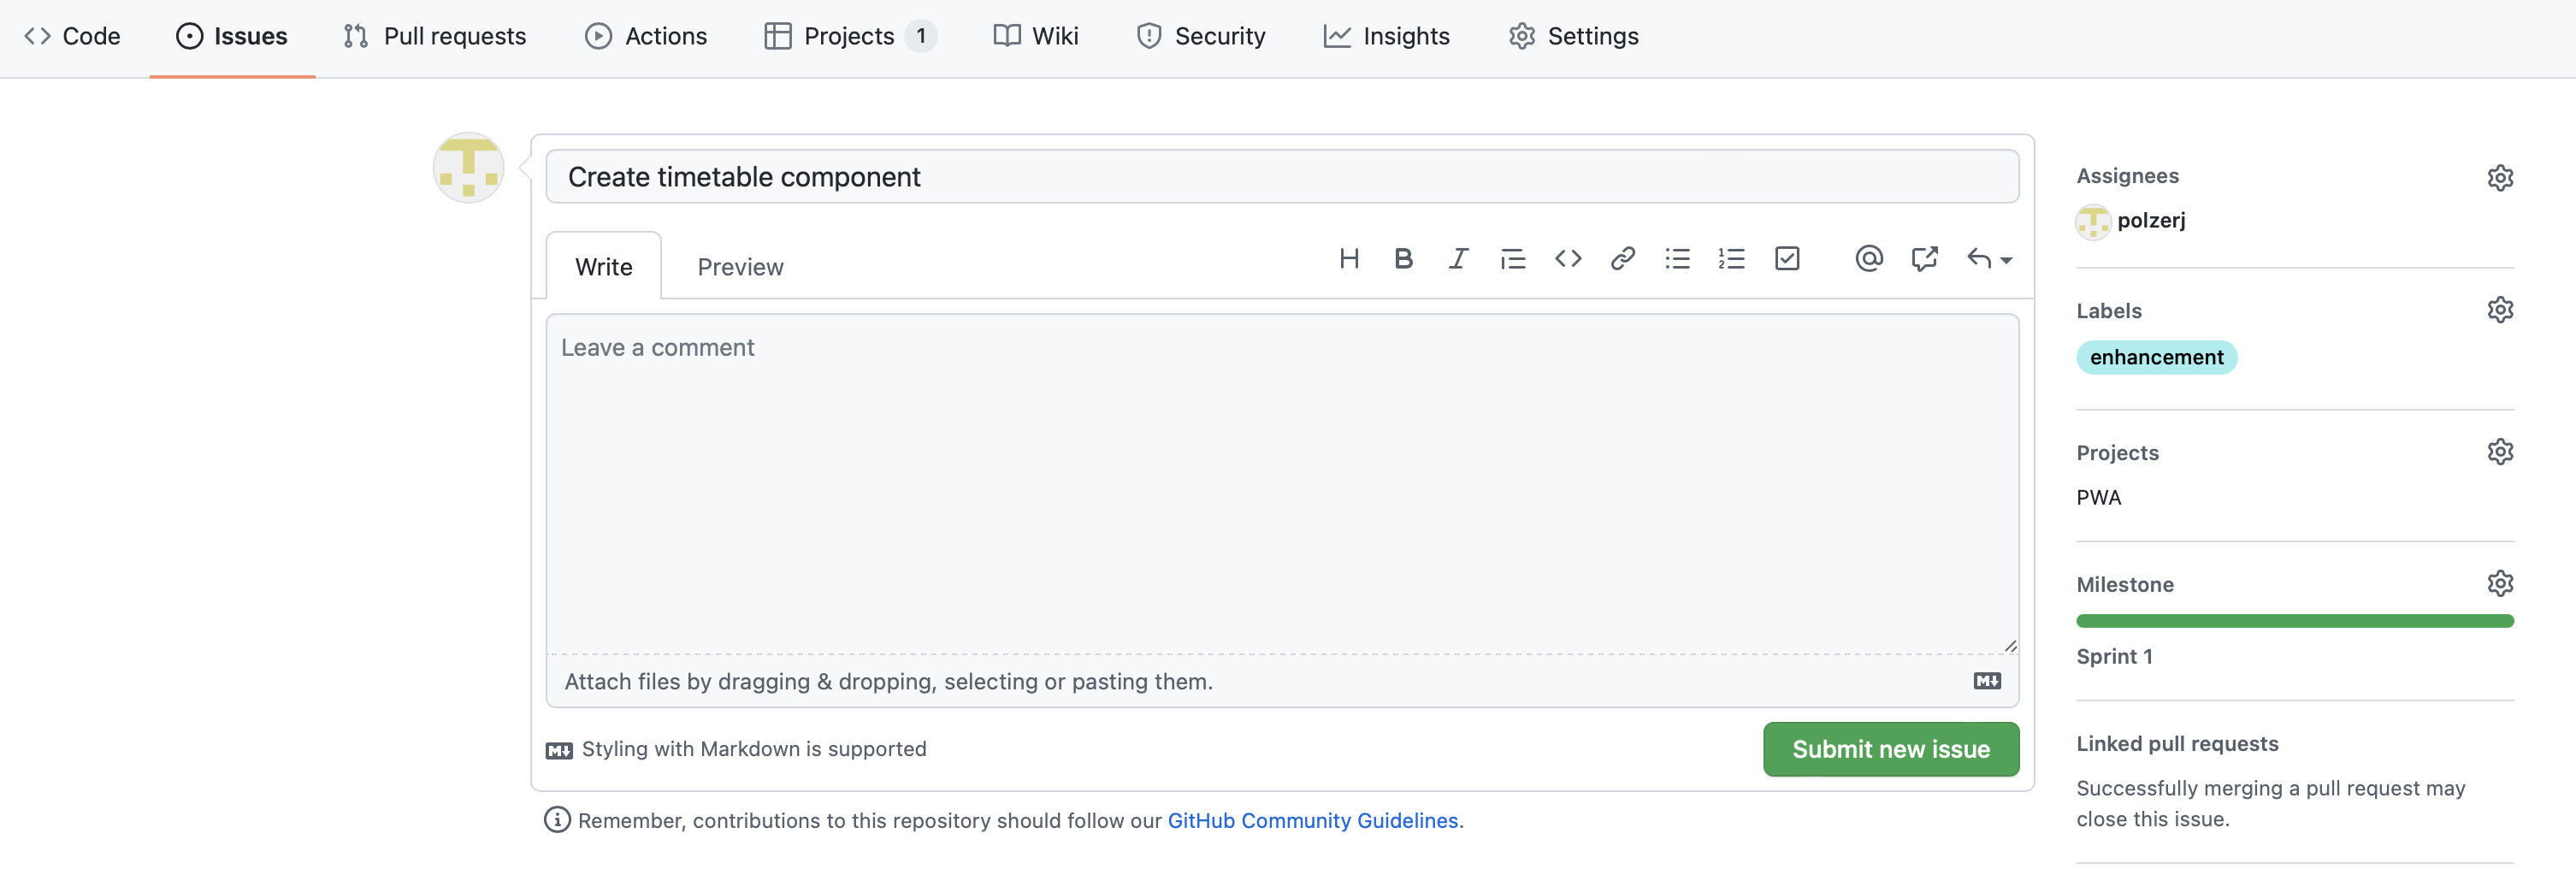
\includegraphics[width=\textwidth]{media/ProjectManagement/CreateIssue.png}
    \caption{Eingabe der Arbeitspaketinformationen (Demo-Bild)}
    \label{fig:createIssue}
\end{figure}

\hthree{Arbeiten an einem Arbeitspaket}

Für jedes Arbeitspaket wird ein eigener Branch mit dem Befehl {\ttfamily git checkout -b <Branch Name>} erstellt. Dabei wird der Name aus der "Issue ID" und dem "Issue"-Titel zusammengesetzt. 

\zb:
{\ttfamily 5-create-timetable-component}

Die "Issue ID" wird aus der Detailansicht eines "Issues" neben dem Titel entnommen (siehe Abbildung \ref{fig:issueInfo}). Dieser Branch kann mit dem Befehl {\ttfamily git push -u origin <Branch Namen>} auf Github hochgeladen werden. 

\begin{figure}[H]
    \centering
    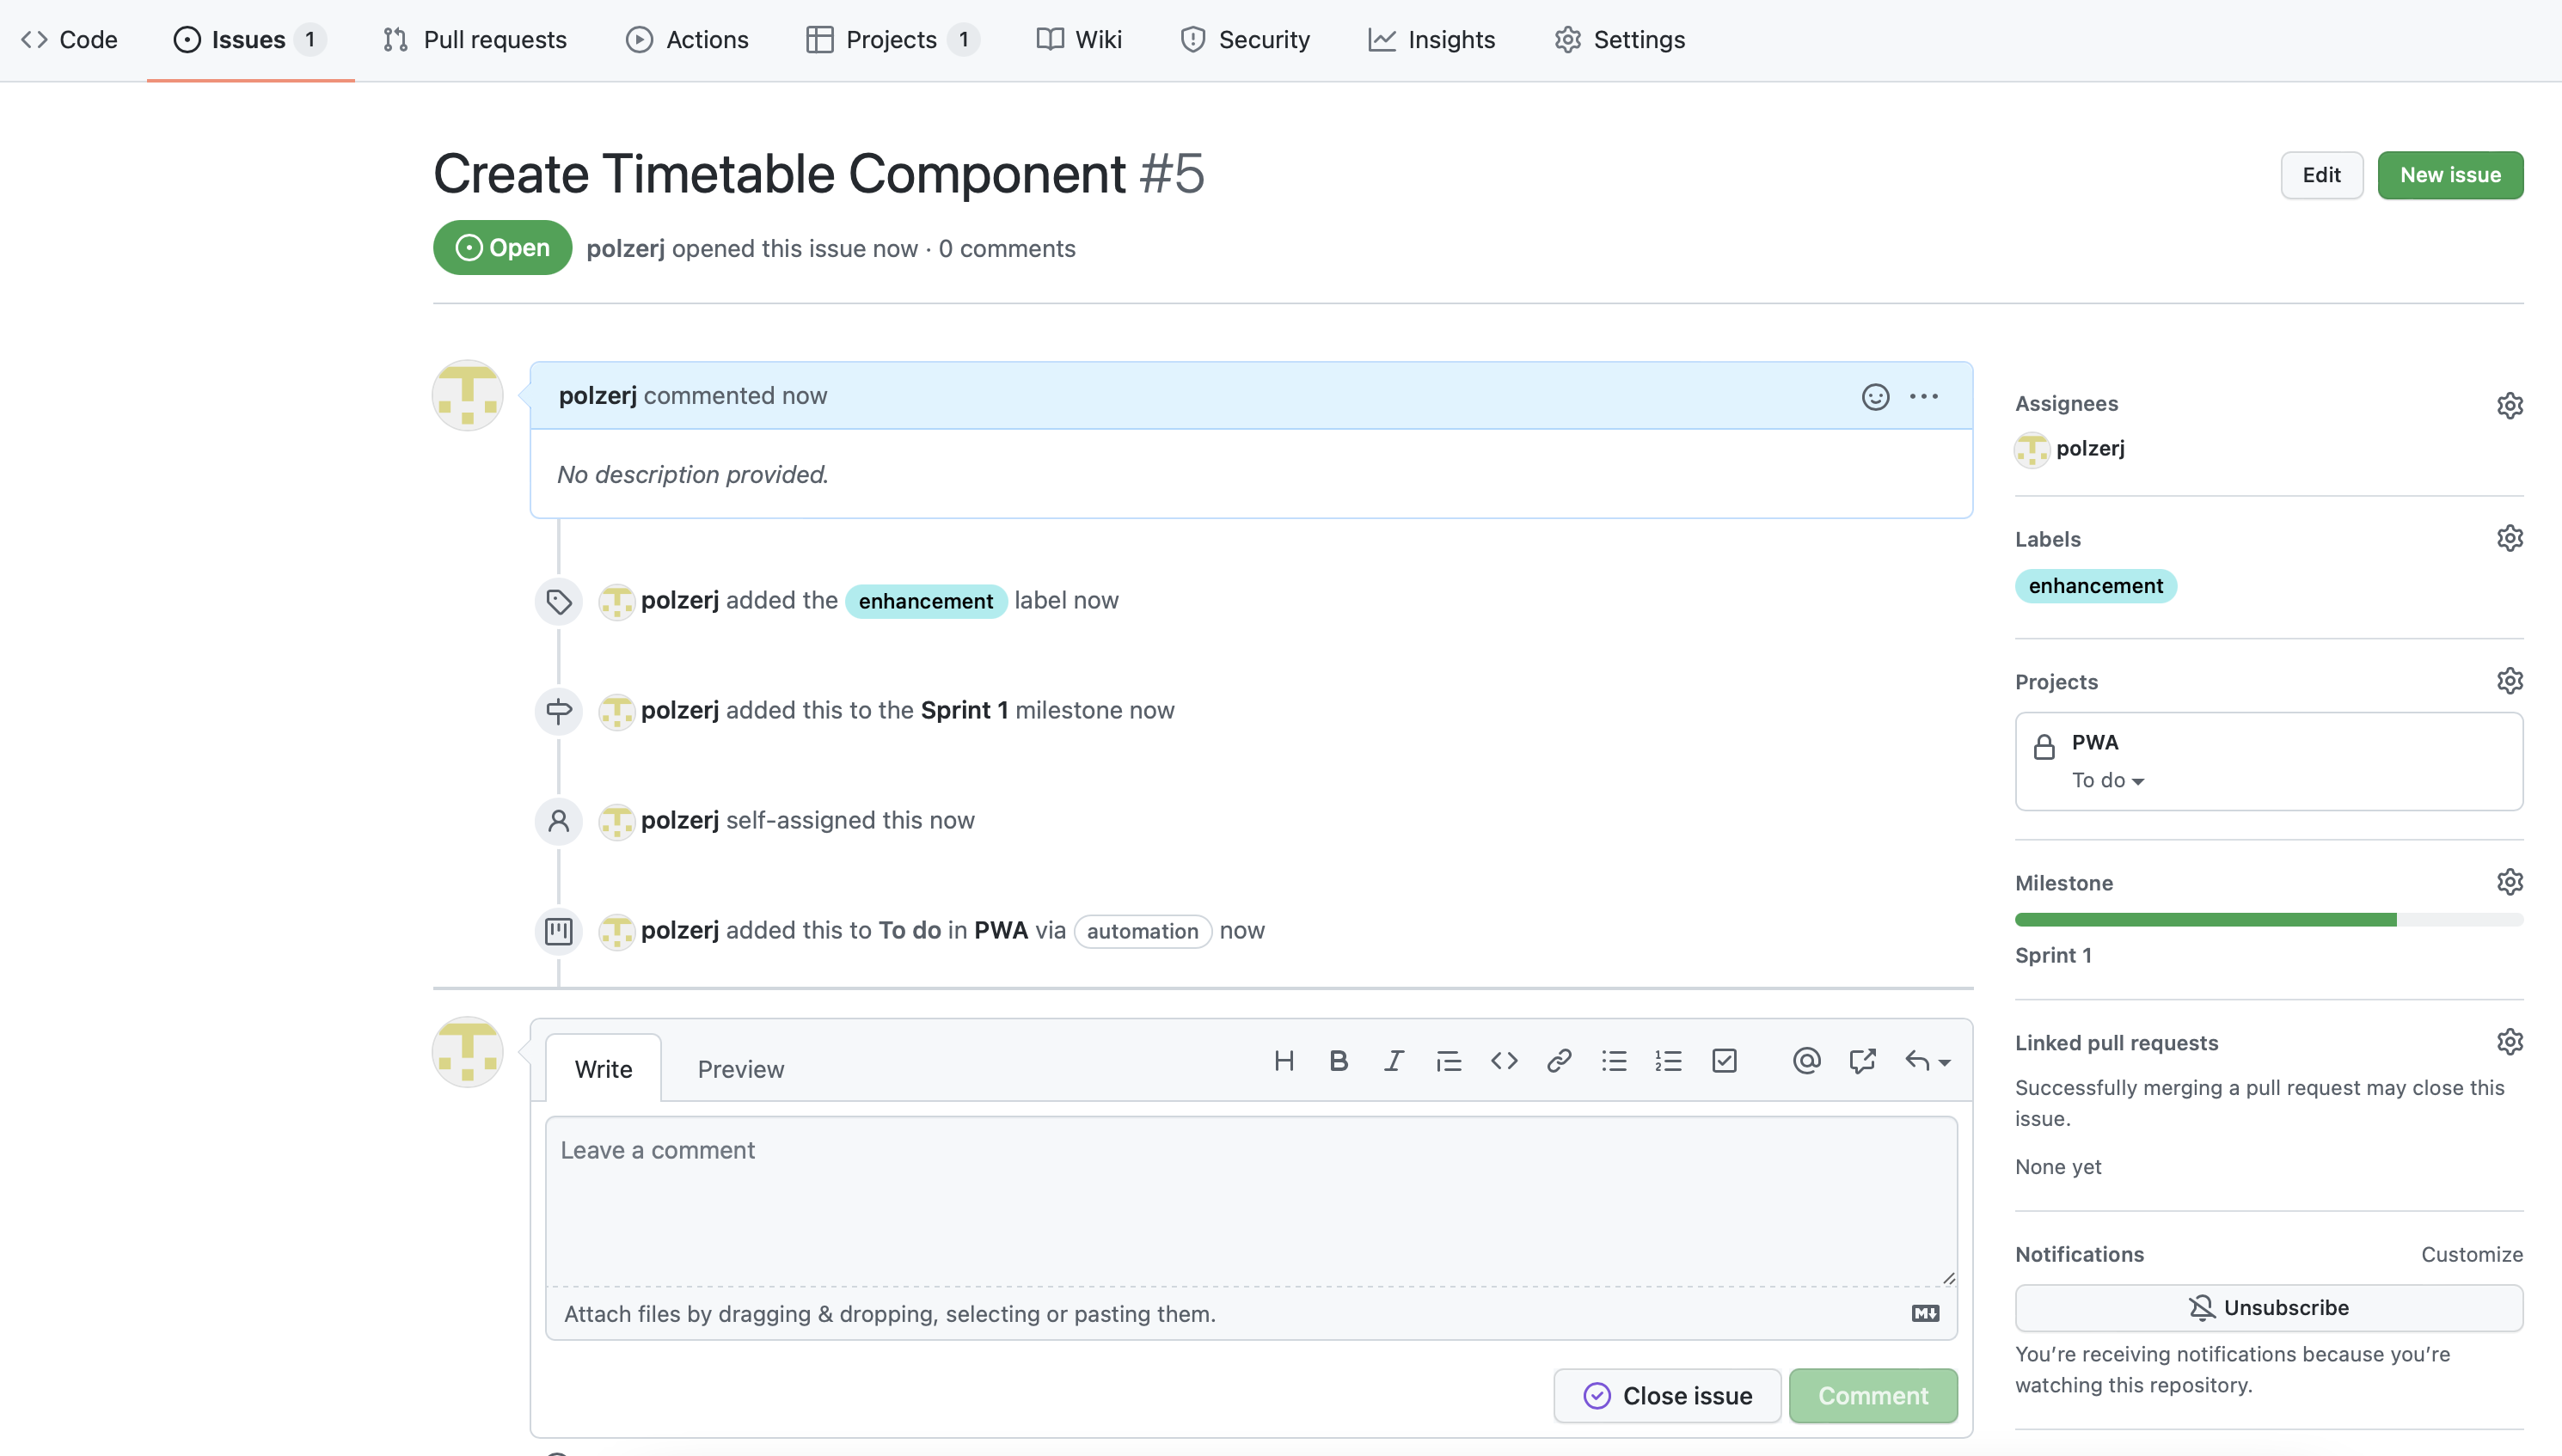
\includegraphics[width=\textwidth]{media/ProjectManagement/IssueInfo.png}
    \caption{Detailansicht "Issue" (Demo-Bild)}
    \label{fig:issueInfo}
\end{figure}

\hthree{Review und Merge}

Wenn die gesamte Funktionalität des Arbeitspakets implementiert ist, wird ein sogenannter "Pull Request" erstellt. Dies wird im "Pull Requests"-Tab gemacht. 

Ein "Pull Request" wird erstellt, um einen Arbeitsbranch eines Issues auf den Branch des jeweiligen Sprints zu integrieren (engl. merge). Davor können allerdings andere Entwickler ("Reviewer") den Code überprüfen und Kommentare hinzufügen. Erst wenn der Code akzeptiert wurde, wird der Merge durchgeführt.

Zunächst muss ausgewählt werden, auf welchen Branch der jeweilige Arbeits-branch zusammengefügt werden soll (siehe Abbildung \ref{fig:createPullRequest}). Dabei wird zunächst immer auf den Branch des jeweiligen Sprints ausgewählt. Erst am Ende eines Sprints wird ein "Pull Request" von dem Branch des Sprints auf den "main"-Branch erstellt.

\begin{figure}[H]
    \centering
    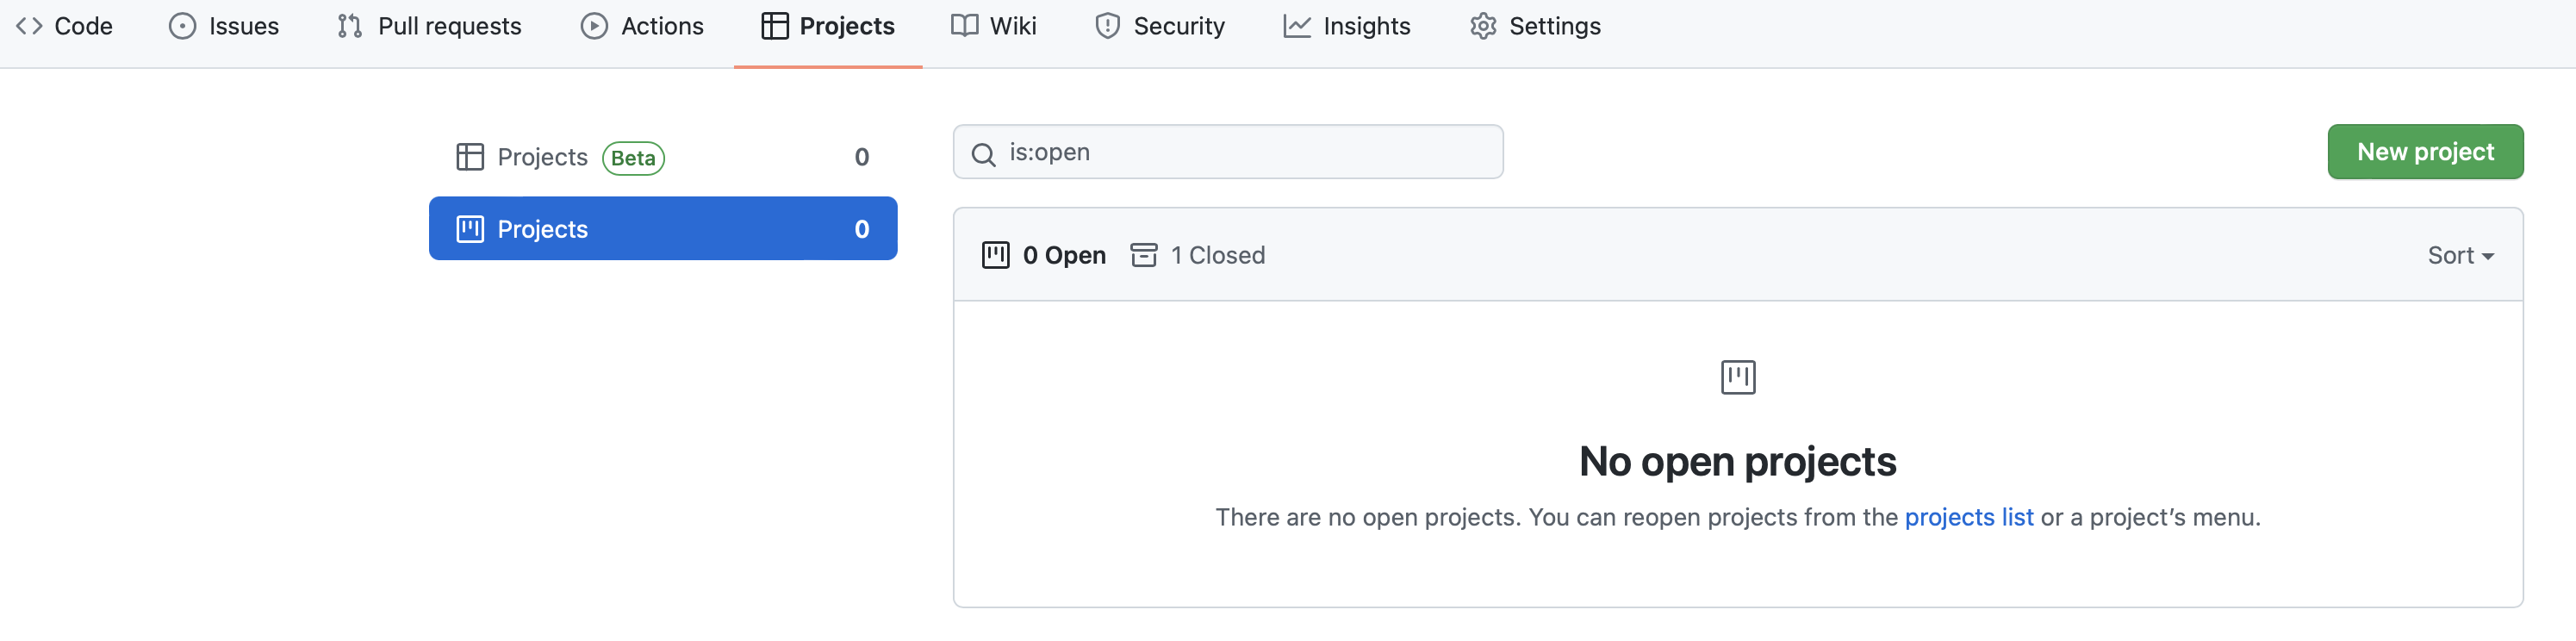
\includegraphics[width=\textwidth]{media/ProjectManagement/CreateProject.png}
    \caption{Erstellen eines "Pull Requests" (Demo-Bild)}
    \label{fig:createPullRequest}
\end{figure}

Um den "Pull Request" zu erstellen, müssen zu den im Issue schon bekannten angegebenen Feldern die Reviewer eingetragen werden. Außerdem muss in der Beschreibung des "Pull Request" "Closes \textless Issue ID\textgreater" angegeben werden (siehe Abbildung \ref{fig:EnterPullRequestInfo}).

\begin{figure}[H]
    \centering
    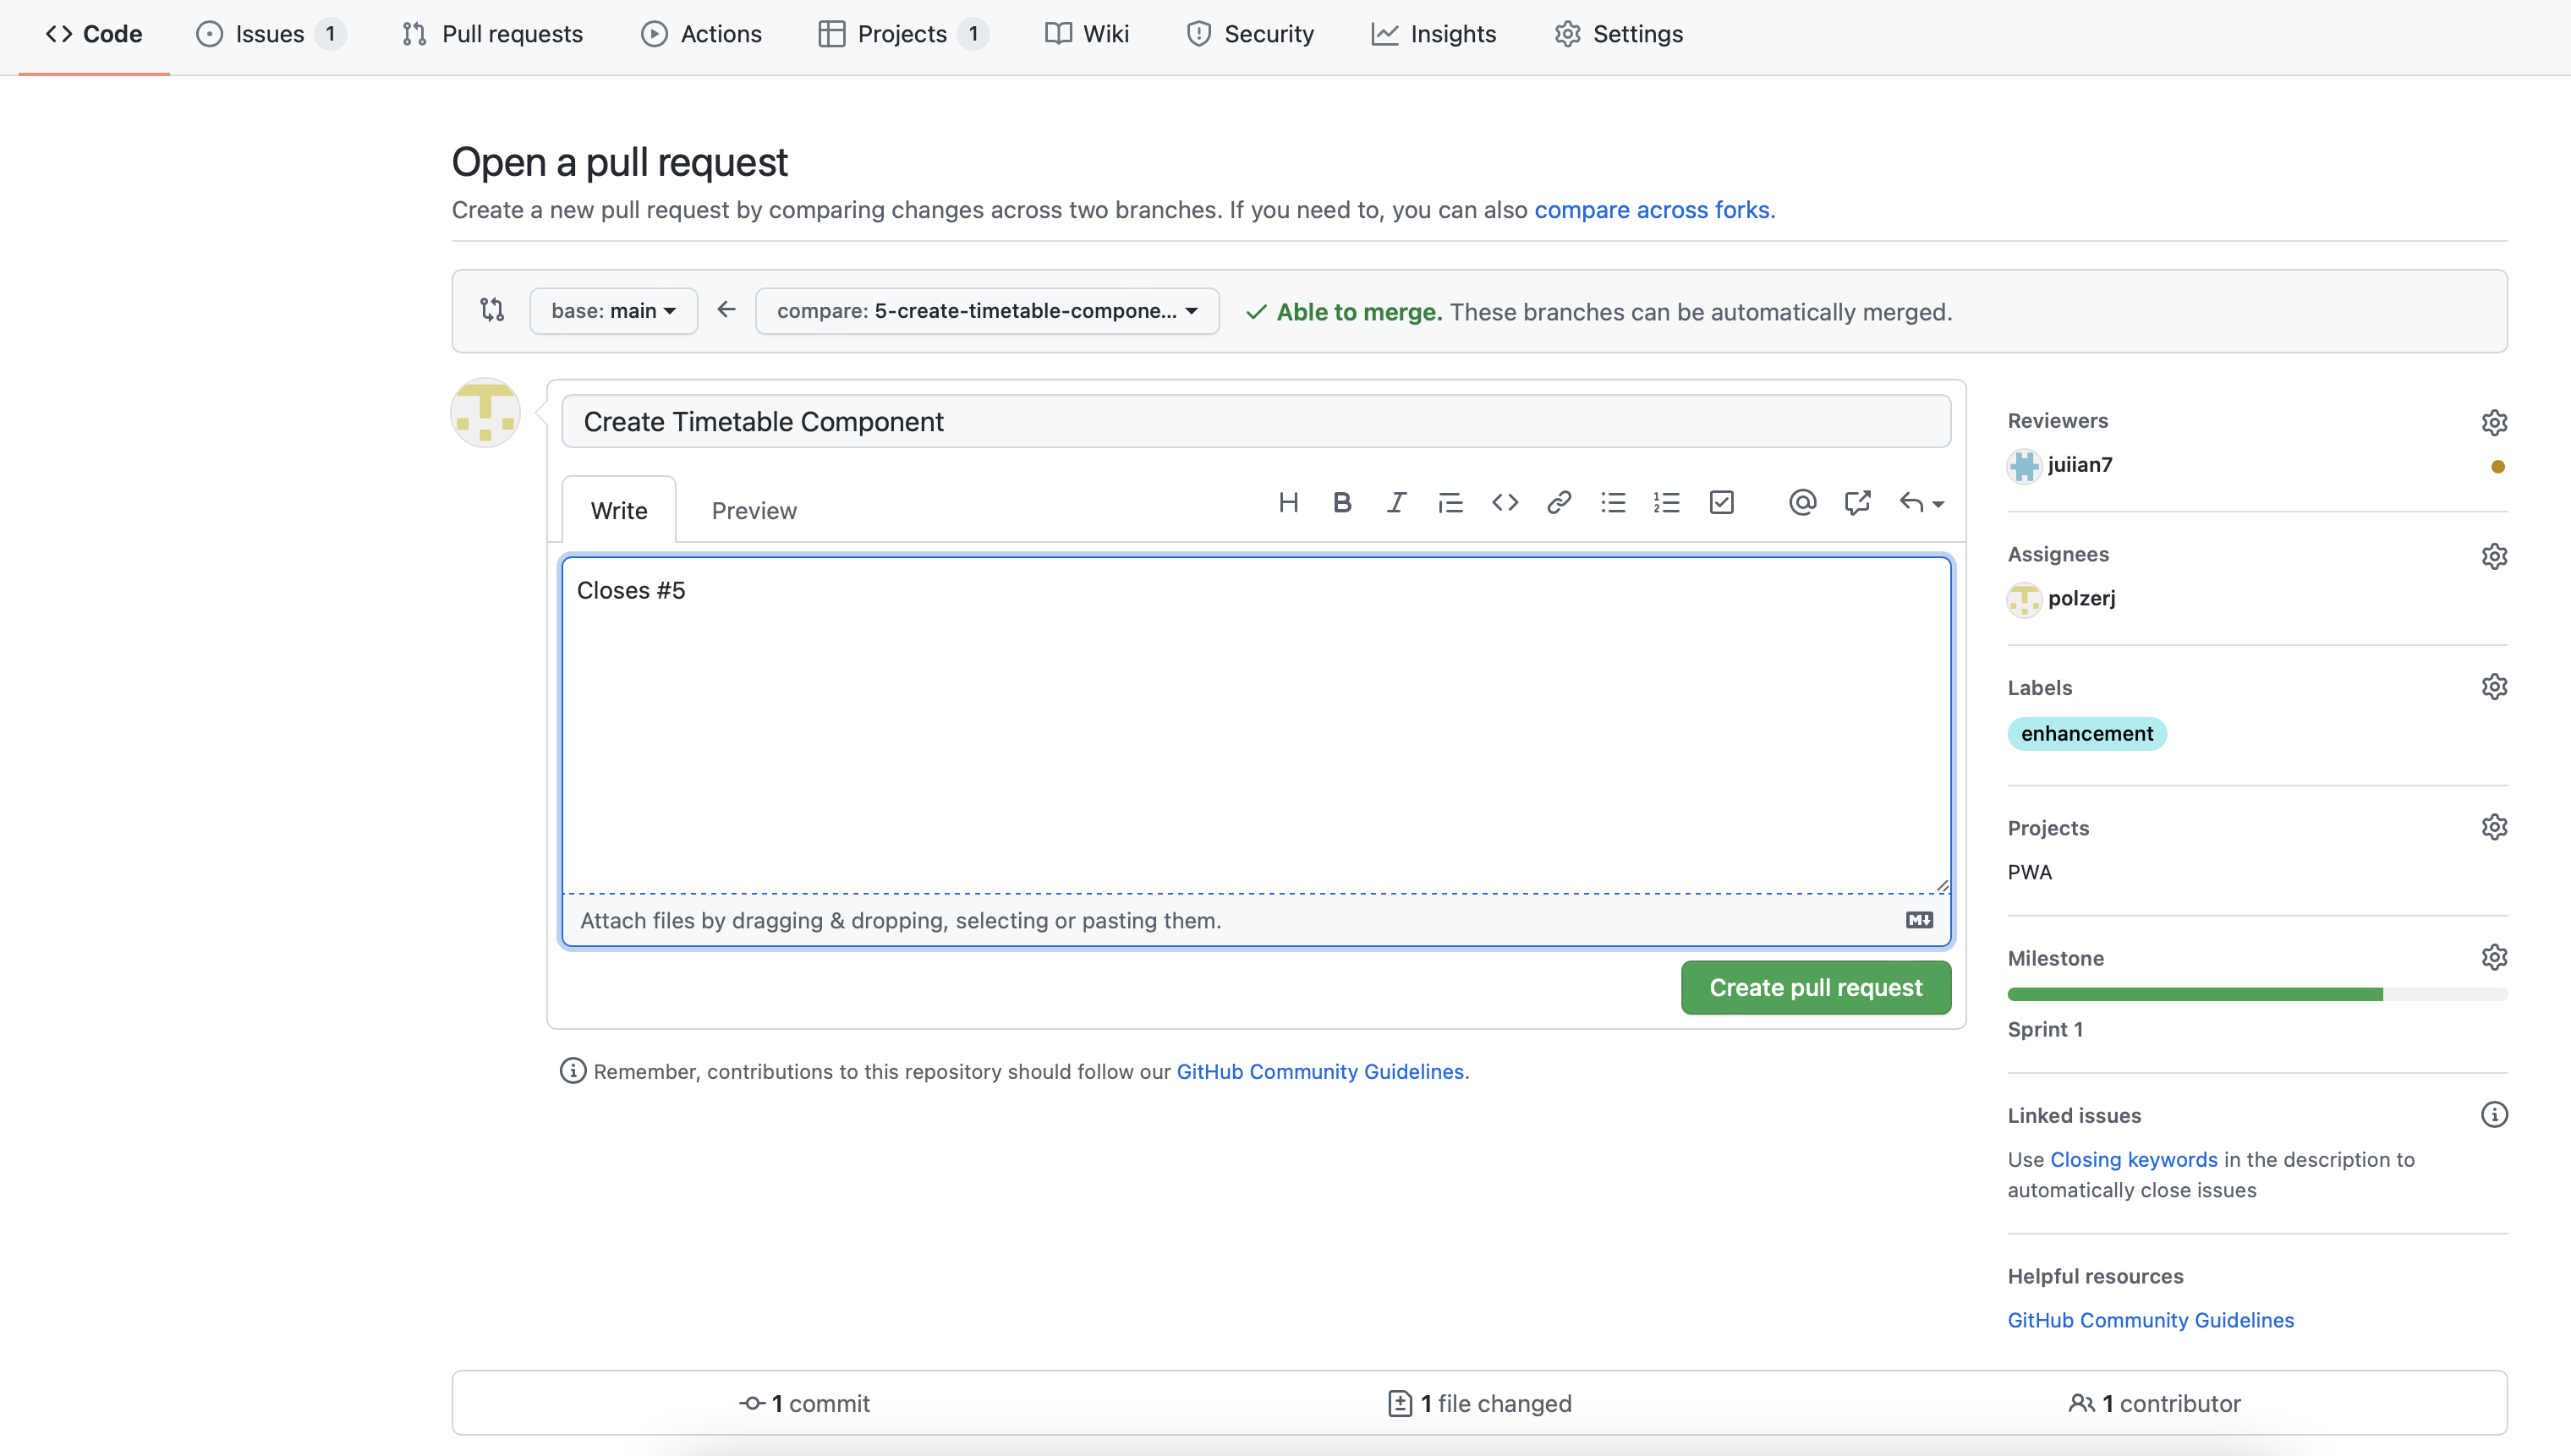
\includegraphics[width=\textwidth]{media/ProjectManagement/EnterPullInfo.png}
    \caption{Setzten der Informationen eines "Pull Requests" (Demo-Bild)}
    \label{fig:EnterPullRequestInfo}
\end{figure}

Die Reviewer können nun im "Files Changed" Tab des "Pull Requests" den Code überprüfen und daraufhin Änderungen anfordern oder den "Pull Request" freigeben. 

Wenn alle Änderungen akzeptiert werden, wird ein "Squash and Merge" durchgeführt (siehe Abbildung \ref{fig:pullInfo}). \\ Dabei werden alle Commit-Nachrichten  zu einem Commit zusammengefasst. Sowohl der "Issue" als auch der "Pull Request" werden automatisch geschlossen und in die "Done"-Spalte verschoben.
\cite{GithubFS}

\begin{figure}[H]
    \centering
    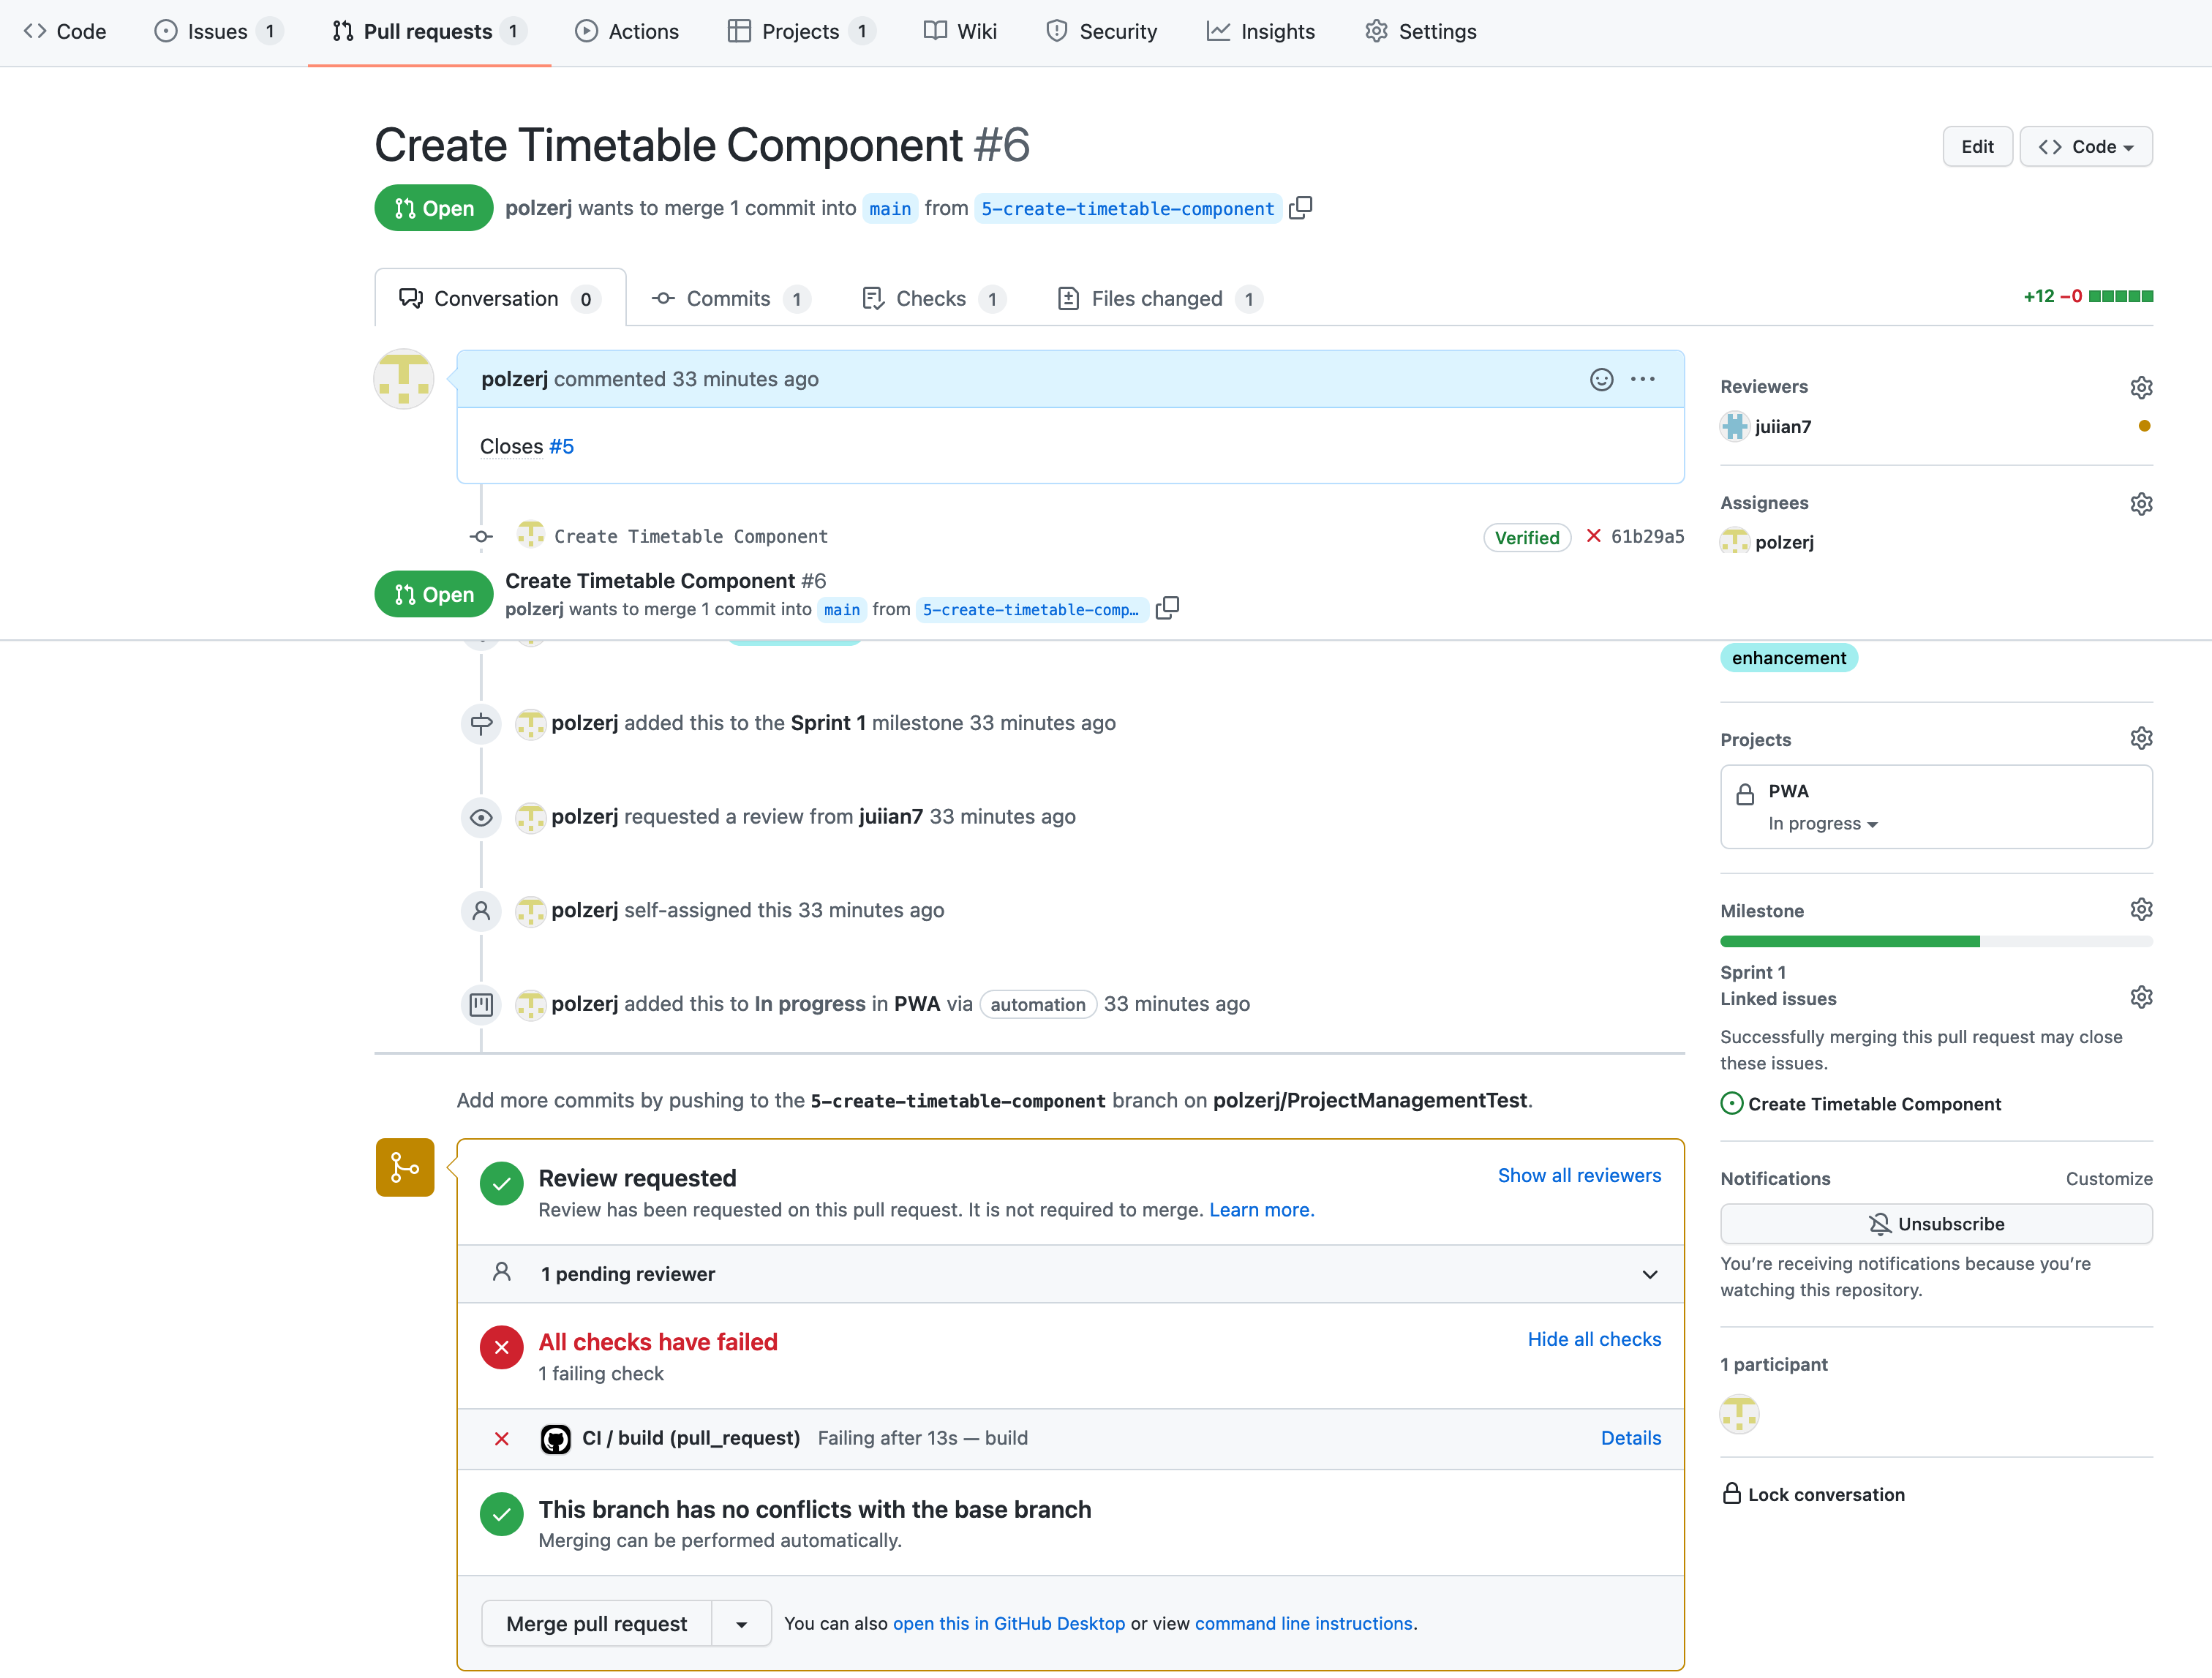
\includegraphics[width=\textwidth]{media/ProjectManagement/PullInfo.png}
    \caption{Detailansicht "Pull Requests" (Demo-Bild)}
    \label{fig:pullInfo}
\end{figure}

\hthree{Wiki}

In dem Wiki-Tab können Informationen über das Projekt abgelegt werden. Diese Seiten werden in Markdown geschrieben. Markdown bietet eine einfache Syntax, um Überschriften, Links, Listen, Code-Auszeichnungen und mehr zu erstellen. In der Seitenleiste kann zu Überschriften navigiert werden (siehe Abbildung \ref{fig:Projektantrag}). Allerdings kann diese Seitenleiste auch selber überschrieben werden.

\begin{figure}[H]
    \centering
    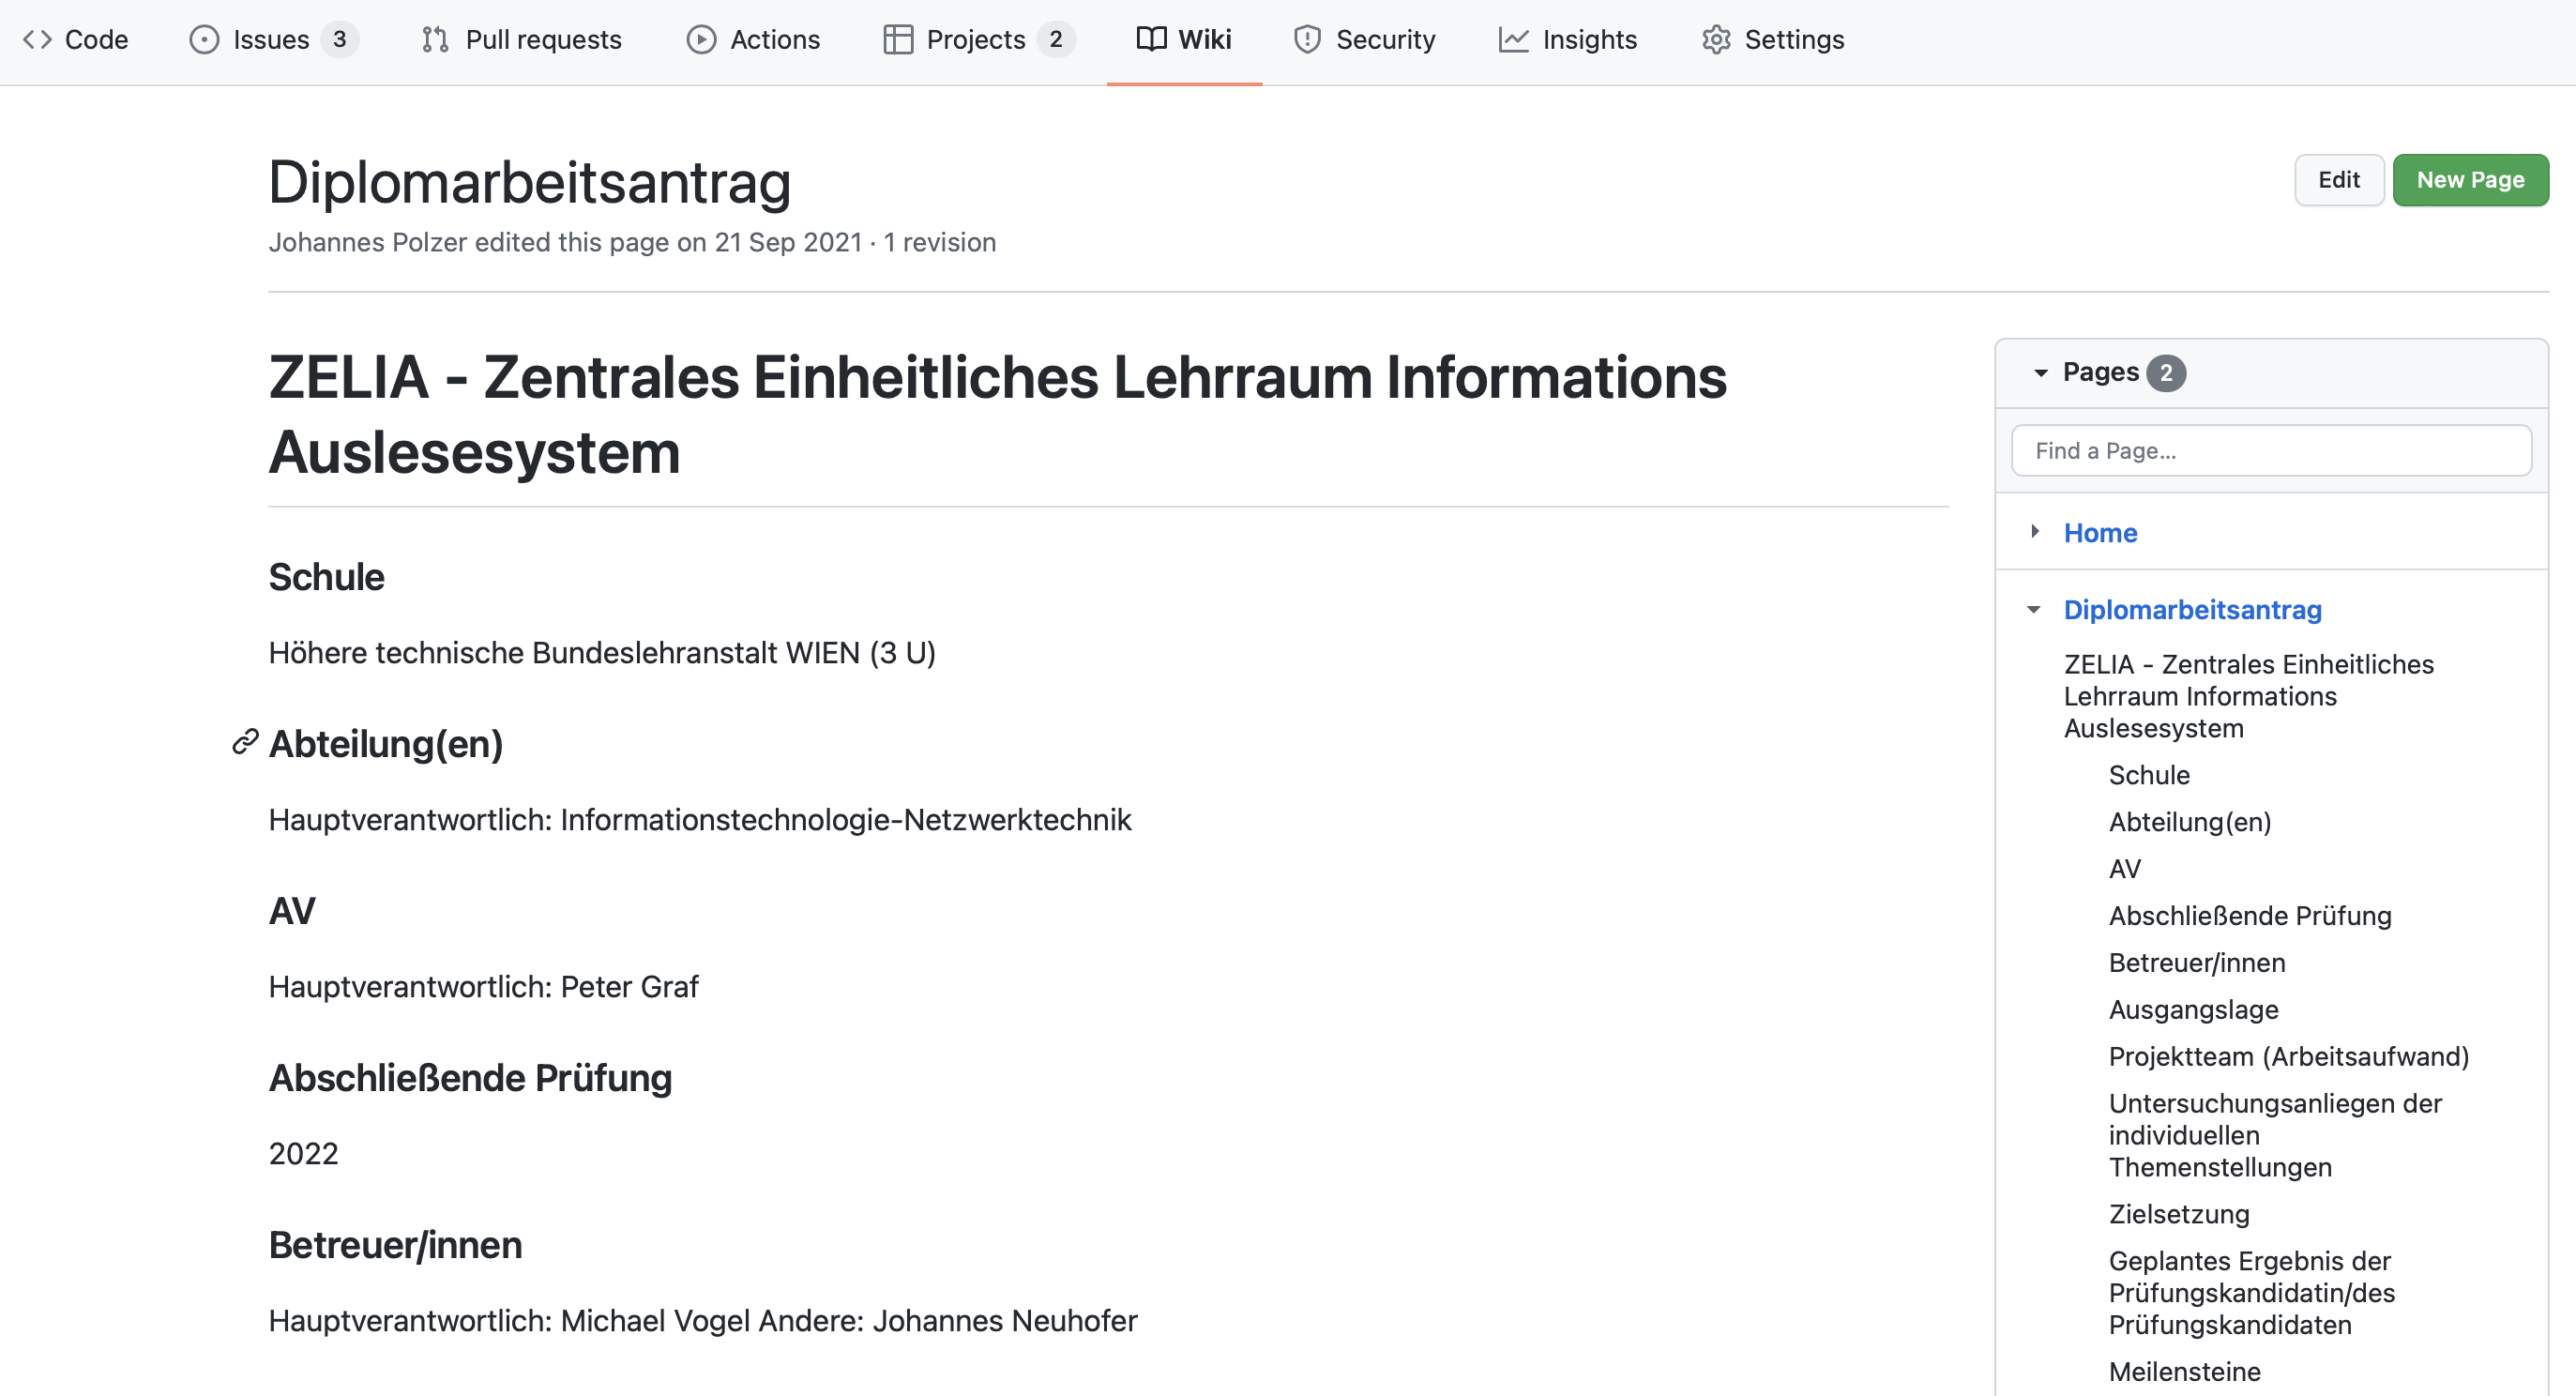
\includegraphics[width=\textwidth]{media/ProjectManagement/Wiki.png}
    \caption{Projektantrag in Github-Wiki}
    \label{fig:Projektantrag}
\end{figure}

Diese Seiten sind auch offline bearbeitbar. Dabei muss lediglich "wiki." vor "git" im Pfad des Repositories eingefügt werden, um das Wiki Repository zu clonen. Das heißt, aus {\ttfamily git@github.com:polzerj/Zelia.git} wird {\ttfamily git@github.com:polzerj/Zelia.wiki.git}. 

\hthree{Insights}

Die Insights ermöglichen es Statistiken über das Projekt auszulesen. Darin sind zum Beispiel die "Contributions" der einzelnen Personen aufgeführt (siehe Abbildung \ref{fig:insights}).

\begin{figure}[H]
    \centering
    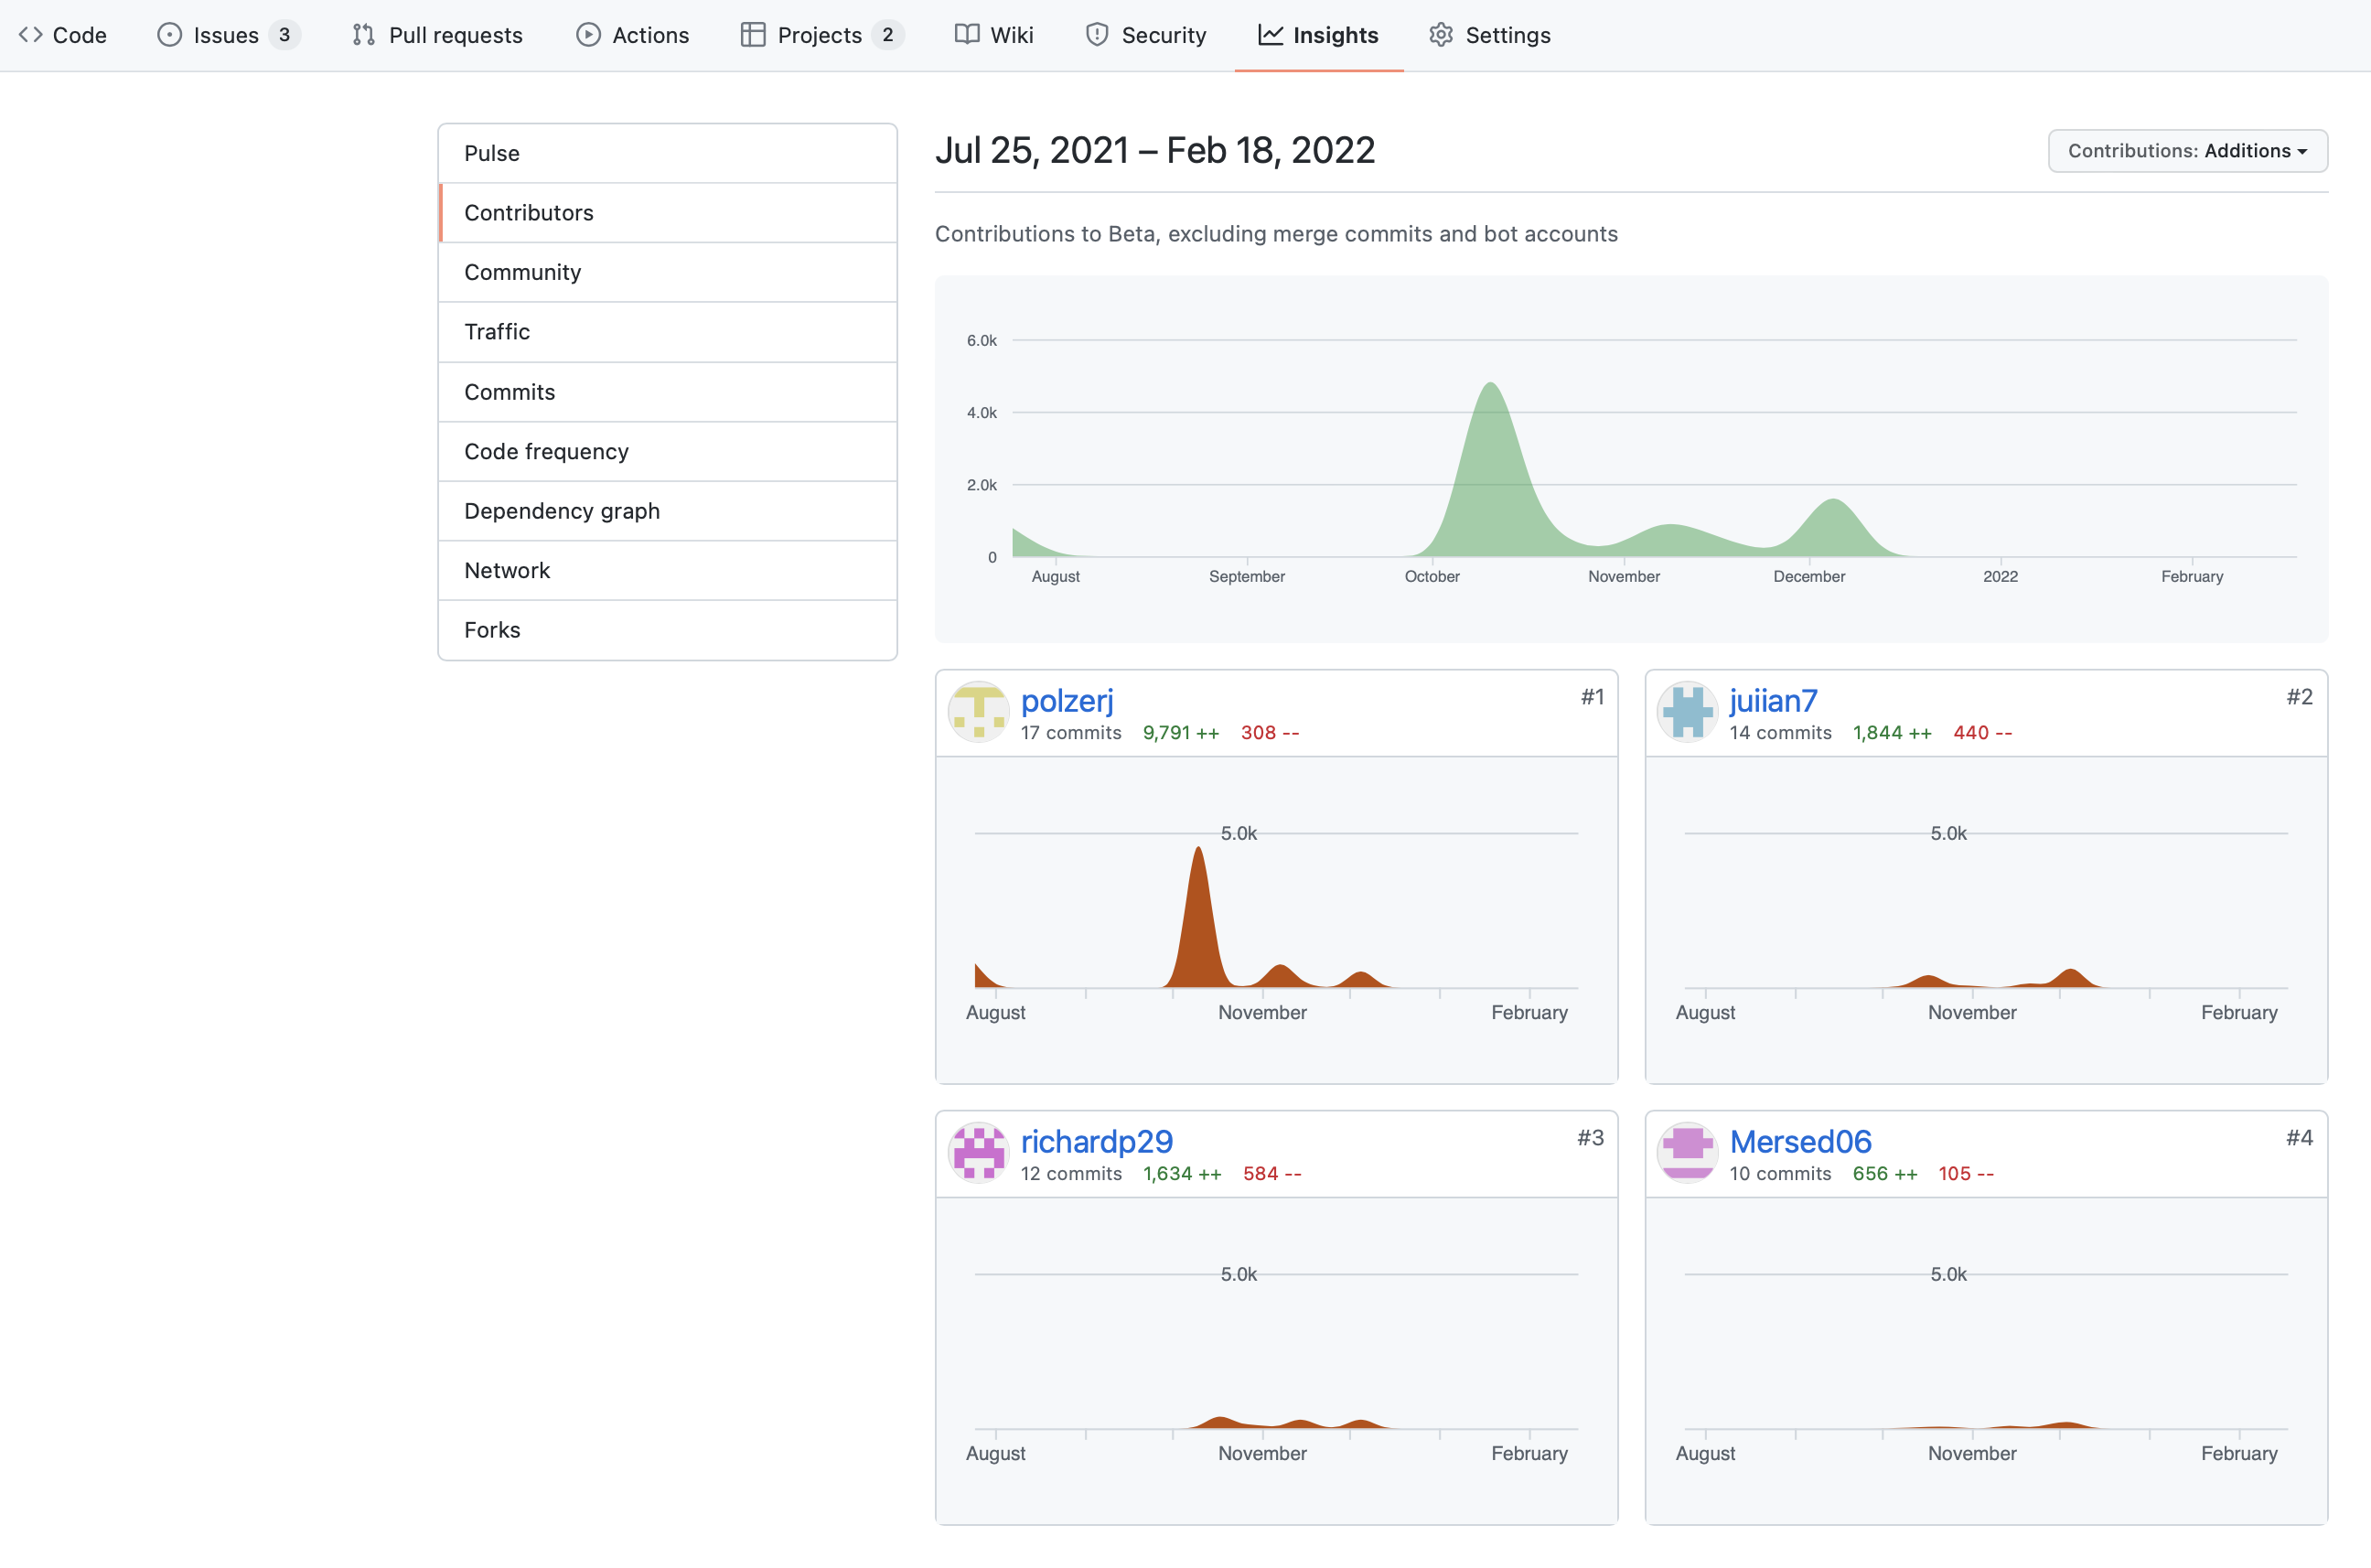
\includegraphics[width=\textwidth]{media/ProjectManagement/Insights.png}
    \caption{Statistik des Entwicklungsbeitrages der einzelnen Projektteilnehmer}
    \label{fig:insights}
\end{figure}